\documentclass[sigconf]{aamas}
\usepackage{amsmath}
\usepackage{balance}
\usepackage{algorithm}
\usepackage{algpseudocode}

% Copyright block from the AAMAS 2027 template; class and layout unchanged.
\makeatletter
\gdef\@copyrightpermission{
  \begin{minipage}{0.2\columnwidth}
   \href{https://creativecommons.org/licenses/by/4.0/}{
\includegraphics[width=0.90\textwidth]{by}}
  \end{minipage}\hfill
  \begin{minipage}{0.8\columnwidth}
   \href{https://creativecommons.org/licenses/by/4.0/}{This work is licensed under a Creative Commons Attribution International 4.0 License.}
  \end{minipage}
  \vspace{5pt}
}
\makeatother
\setcopyright{ifaamas}
\acmConference[AAMAS 2027]{Proc.\@ of the 26th International Conference
on Autonomous Agents and Multiagent Systems (AAMAS 2027)}{3--7 May 2027}{Hanoi, Vietnam}{M.~Baldoni, F.~Fang, W.~Yeoh, N.~Yorke-Smith (eds.)}
\copyrightyear{2027}
\acmYear{2027}
\acmDOI{}
\acmISBN{}
% Fill in the actual identifier after registering the abstract on OpenReview.
\InputIfFileExists{submission-id.tex}{}{\acmSubmissionID{}}
\submissionType{Research Paper Track}
\title[RAG-ConGuard: Coalition-Level Evidence Filtering]{RAG-ConGuard: Coalition-Level Evidence Filtering and Safety--Availability Trade-offs in Poisoned RAG}
\author{Jinsong Yang}
\email{yangjinsong@gs.zzu.edu.cn}
\orcid{0009-0009-3038-3667}
\affiliation{%
  \institution{Zhengzhou University}
  \city{Zhengzhou}
  \state{Henan}
  \country{China}}

\author{Enhao Zhang}
\email{zhangeh@zzu.edu.cn} % TODO: confirm actual email.
\affiliation{%
  \institution{Zhengzhou University}
  \city{Zhengzhou}
  \state{Henan}
  \country{China}}

\author{Zhihua Wang}
\authornote{Corresponding author.}
\email{zhwang@zzu.edu.cn} % TODO: confirm actual corresponding-author email.
\affiliation{%
  \institution{Zhengzhou University}
  \city{Zhengzhou}
  \state{Henan}
  \country{China}}

\renewcommand{\shortauthors}{Yang et al.}

\begin{abstract}
Knowledge-grounded agents can consume several retrieved passages that repeat the same attacker-chosen answer. Filtering these passages jointly offers a way to reduce their collective presence, but aggressive filtering can also deprive a generator of useful evidence. We present RAG-ConGuard, an inference-time evidence filter that groups semantically related passages, summarizes their signed relations, and predicts risk at the group level. Two context selectors expose the trade-off between removing suspicious evidence and retaining a nonempty context. On a development-exposed, 60-query attacked evaluation spanning three question-answering datasets, the availability-oriented configuration reduces attack success from 83.3\% to 48.3\%, with 10.0\% refusal. A more aggressive configuration reduces attack success to 18.3\% with 45.0\% refusal; a TrustRAG adaptation achieves 15.0\% with 48.3\% refusal, so these results do not establish dominance over that baseline. Four-variant, three-seed ablations show no aggregate benefit from the auxiliary graph-support Impact feature at the availability point. Generation-distribution probes, including complete evidence removal, also provide insufficient evidence to validate Impact as a generation-effect proxy. Clean-answer scores are unchanged on 300 gold-available HotpotQA queries, while clean refusal increases on other datasets. The evidence supports coalition-level filtering as a configurable safety--availability trade-off, with limited generalization evidence and no validated causal attribution claim.
\end{abstract}
\keywords{retrieval-augmented generation, knowledge poisoning, evidence filtering, trustworthy agents, abstention}
\ccsdesc[500]{Security and privacy}
\ccsdesc[300]{Computing methodologies~Natural language generation}

\begin{document}
\maketitle

\section{Introduction}
Retrieval-augmented generation (RAG) supplies language models with external evidence for knowledge-intensive tasks~\cite{rag}. When a knowledge-grounded agent relies on that evidence, an attacker who can insert passages into the corpus gains an indirect influence channel. Targeted knowledge-corruption attacks exploit this channel by promoting an incorrect answer through retrieved text~\cite{poisonedrag}. The relevant intervention point is therefore not only the model's final response: it is also the evidence that the model is allowed to read.

Several passages may express the same misleading proposition. Their repetition can survive the deletion of an individual passage, motivating a filter that operates on groups. However, semantic agreement also occurs among legitimate passages. Group size and internal agreement alone cannot establish malicious coordination, and several agreeing documents need not represent independent sources. A practical filter must balance removing suspicious groups against retaining sufficient evidence to answer.

RAG-ConGuard addresses this evidence-selection problem using a compact representation of the retrieved context. It extracts one short excerpt per passage, groups excerpts by semantic similarity subject to a pairwise contradiction check, and computes structural features from a signed natural-language-inference (NLI) graph. A small supervised classifier assigns a risk score to each eligible group, termed an \emph{evidence coalition}. One selector removes all coalitions above a risk threshold; another preserves a minimum number of passages. Here, a coalition is a group of evidence items, not a collection of autonomous agents or a game-theoretic solution concept.

The central empirical question is whether this grouping and selection pipeline offers a useful operating point. A separate question is what explains its behavior. We distinguish these questions because a successful filter does not automatically validate every input feature. In particular, an auxiliary \emph{Impact} score measures how graph-derived evidence support changes when a coalition is removed. This is a counterfactual calculation on a deterministic graph operator. Its relation to the generator's behavior must be measured separately.

Filtering reduces attack success but also affects availability. The retained-context point still allows 29 attacks among 60 queries. The aggressive point allows 11 attacks but refuses 27 queries. The TrustRAG adaptation allows nine attacks and refuses 29 queries. These outcomes support configurable filtering, without establishing superiority over that baseline. The ablations and probes do not validate Impact as a generation-effect proxy.

The contributions are threefold:
\begin{itemize}
\item An inference-time coalition-level filter combining semantic groups, graph features, and policies for context retention, with a clear separation between risk estimation and evidence selection.
\item Measurements of attack success, answer matching, and refusal on three datasets, with two operating points, generator transfer, and a partially labeled clean evaluation.
\item A controlled analysis that separates Impact's classifier input from its eligibility-rule dependency, and compares graph-support changes with generation-distribution probes and available same-size deletion controls.
\end{itemize}
The experiments isolate evidence use in single-turn QA. Planning, tool use, multiagent coordination, and long-horizon task completion are not evaluated. The attacked evaluation queries were examined during development; results are consequently exploratory rather than an independent confirmation of generalization.

\section{Related Work}
\paragraph{Corpus poisoning and service availability.}
PoisonedRAG formulates targeted knowledge corruption through a small number of injected passages~\cite{poisonedrag}. We use the corresponding target-answer threat model with a project-specific synthetic attack construction, without claiming to reproduce every attack optimization in that work. SafeRAG broadens evaluation to several security failure modes, including conflicting evidence and denial of service~\cite{saferag}. These distinctions motivate reporting refusal separately from target-answer success: a defense can reduce the latter while making the system less useful. Our experiment covers targeted answer poisoning, not the full SafeRAG benchmark.

\paragraph{Filtering untrusted evidence.}
TrustRAG uses clustering and a subsequent self-assessment process to distinguish malicious information and reconcile retrieved and internal knowledge~\cite{trustrag}. ShieldRAG uses adversarial generation and evaluation components to defend against untrusted knowledge~\cite{shieldrag}. Our method instead learns a small classifier over group features and applies an explicit context-retention policy. This difference does not imply that existing defenses ignore context relations. Our B5 comparison is an adaptation of TrustRAG to the project pipeline, and its measured operating point is not a refusal-matched comparison against the original system.

\paragraph{Evidence representation and attribution.}
The retriever uses dense embeddings from the BGE family~\cite{bge} alongside sparse retrieval; the datasets are drawn from retrieval-oriented question-answering resources~\cite{beir}. NLI relations provide an approximate signed structure over excerpts~\cite{nlimodel}. Such relations are not factuality certificates or measurements of source independence. Likewise, deleting nodes from a support graph and deleting passages from a generator's context are different interventions. We use teacher-forced distribution comparisons to examine their association, without identifying a causal effect on answer correctness or autonomous behavior.

\section{Problem and Threat Model}
Let $q$ be a query, $\mathcal{K}$ a corpus, and $D=(d_1,\ldots,d_n)$ the ranked retrieved context. A generator $f_\theta$ produces an answer from $q$ and a selected subsequence $D'\subseteq D$. The attacker inserts a set $P$ of passages into $\mathcal{K}$ to induce a chosen incorrect answer $y^{\mathrm{adv}}_q$. The attacker controls inserted text but not the defender's model weights, system prompt, or scoring labels. The evaluated budget is five injected passages per target query, and retrieval returns $n=5$ passages. The defender observes the query and retrieved text, but does not use either the correct answer or $y^{\mathrm{adv}}_q$ to construct runtime features.

We examine three outcomes: production of the target answer, production of a reference-matching answer, and refusal. All rates use the full evaluated query set as their denominator. Refusal is a loss of availability in this task, even when it prevents an attack. Conversely, a non-refusal is not automatically a correct answer. A document-retention floor constrains evidence deletion only; it guarantees neither correctness nor a bound on generator refusal.

The attacker's passages may form a semantically coherent cluster, but no trusted provenance signal is assumed. Our use of ``coalition'' describes this measurable grouping. It does not establish common authorship, independent corroboration, or actual cooperation between document sources. The reported attacks are fixed constructions. Detector-aware adaptive robustness is outside the validated experimental scope.

\section{Coalition-Level Evidence Filtering}
\label{sec:method}
\subsection{Excerpts, Relations, and Grouping}
Each retrieved passage contributes its leading 220 characters as one excerpt $c_i$. This truncation does not extract claims based on the query and can omit relevant text. BGE embeddings $e_i$ represent these excerpts. A cross-encoder NLI model assigns support, contradiction, or neutral relations to directed excerpt pairs. The resulting graph is $G=(V,E^+,E^-)$, with neutral relations discarded. The graph pipeline also supports a numerical-conflict check; the reported configuration uses NLI-based relation extraction rather than an LLM judge.

Grouping and signed feature extraction use distinct relations. The semantic grouping graph joins $i$ and $j$ when $\cos(e_i,e_j)\geq0.85$ and the pair is not marked contradictory. Its connected components are coalition candidates. They are not simply positive-NLI connected components. Transitive connectivity can still place an indirectly connected contradictory pair in the same component, so a coalition need not be globally consistent. The positive-edge grouping variant appears as comparator A in the experiments.

For a coalition $C$ of size $m\geq2$, define $U^+$ and $U^-$ as the deduplicated unordered versions of $E^+$ and $E^-$. Two structural features are
\begin{align}
h(C)&=\frac{|\{\{i,j\}\in U^+:i,j\in C\}|}{\binom{m}{2}},\\
r(C)&=\frac{|\{\{i,j\}\in U^-:|\{i,j\}\cap C|=1\}|}{m}.
\end{align}
The cohesion $h$ counts internal support; $r$ counts crossing contradictions per member. In particular, $r$ is not the probability of refutation or support for a competing answer. Deduplicating edges here prevents double counting directed NLI pairs. The support operator below retains directed relations.

\subsection{Auxiliary Graph-Support Impact}
\label{sec:impact}
The graph operator assigns nonnegative weights through four iterations, starting from $p_i^{(0)}=1$:
\begin{equation}
p_i^{(t+1)}=\frac{0.5+\sum_{(j,i)\in E^+}p_j^{(t)}}{1+2\sum_{(j,i)\in E^-}p_j^{(t)}},\quad t=0,\ldots,3.
\end{equation}
These finite-iteration weights are not normalized probabilities, and no convergence property is assumed. The two excerpts most similar to the query serve as fixed support candidates $\mathcal{A}_q$. They are text excerpts, not oracle answer labels. With their embeddings $e_a$, define
\begin{equation}
s_G(a)=\sum_{i\in V}p_i^{(4)}\max\{0,\cos(e_i,e_a)\}.
\end{equation}
Removing $C$ deletes its vertices and incident relations. Weights are recomputed on $G\setminus C$ with fixed candidates. Define the maximum support as $Z_G=\max_{a\in\mathcal{A}_q}s_G(a)$. The feature is
\begin{equation}
I(C)=\begin{cases}
\displaystyle\max\left\{0,\frac{\max_{a\in\mathcal{A}_q}[s_G(a)-s_{G\setminus C}(a)]}{Z_G}\right\},&Z_G>0,\\
0,&Z_G=0.
\end{cases}
\label{eq:impact}
\end{equation}
This is a normalized support decline, not an answer-margin change. Empty graphs have zero support. Hence complete removal gives $I(C)=1$ whenever $Z_G>0$, irrespective of how the language model responds. This degeneracy is relevant to interpreting the probe experiment.

\subsection{Risk Estimation and Eligibility}
The main classifier, C4, takes $x_C=(m,h(C),r(C),I(C))$. External corroboration and the derived ``control'' quantity from an earlier feature representation are not inputs. A StandardScaler and an MLP with hidden layers $(16,8)$ and maximum 500 training iterations are fitted on training coalition examples. The binary label is one when at least 80\% of a coalition's passages are injected. Other examples form the negative class, which can include mixed groups; it is not equivalent to a verified-benign class. Poisoning annotations are used for training and evaluation, not runtime inference.

The original eligibility rule is
\begin{equation}
g(C)=\mathbf{1}\{m\geq2\}\mathbf{1}\{h(C)>0\ \lor\ I(C)>0\}.
\label{eq:gate}
\end{equation}
Only eligible coalitions are scored and considered for deletion. Singletons are exempt, creating a deliberate blind spot for isolated malicious passages. Importantly, removing $I$ from $x_C$ alone does not remove its influence through $g$; Section~\ref{sec:ablation} isolates the two dependencies.

\subsection{Context Selection}
Let $\rho_C\in[0,1]$ denote the classifier score. The \emph{S0} selector removes every eligible coalition with $\rho_C\geq\tau$. If the resulting context is empty, the system returns an explicit refusal; a generator can also refuse with nonempty evidence.

The \emph{S2} selector sorts eligible coalitions by decreasing $\rho_C$ once, using the existing order for ties, and applies Algorithm~\ref{alg:s2}. Its retention floor is $L=\max\{1,\lfloor\lambda n\rfloor\}$ for nonempty $D$, with $\lambda=1$ retaining all passages. When the next coalition would violate this floor, the procedure stops; it does not skip that coalition and seek a smaller one. Risk scores are not recomputed after a deletion. The output preserves the original relative document order.

\begin{algorithm}[t]
\caption{S2: coalition removal with a retention floor}
\label{alg:s2}
\begin{algorithmic}[1]
\Require Ranked context $D$; eligible coalitions; scores $\rho$; $\lambda,\tau$
\State $D'\gets D$; $L\gets\max\{1,\lfloor\lambda|D|\rfloor\}$
\For{$C$ in descending score order}
  \If{$\rho_C<\tau$}
    \State \textbf{break}
  \EndIf
  \If{$|D'\setminus\mathrm{docs}(C)|<L$}
    \State \textbf{break}
  \EndIf
  \State $D'\gets D'\setminus\mathrm{docs}(C)$
\EndFor
\State \Return $D'$ in original retrieval order
\end{algorithmic}
\end{algorithm}

The retention constraint exposes an unavoidable failure case: if all retrieved passages form one coalition, S2 cannot delete it while keeping a nonempty context. Even a perfect risk score cannot remove that coalition under this policy. Thus availability preservation can dominate feature quality at an operating point. S0 avoids this particular restriction at the cost of possible empty-context refusals. Pairwise relation extraction scales quadratically in the number of excerpts; the present experiments use only five. The graph calculations do not require online generation probes.

\section{Experimental Protocol}
\label{sec:protocol}
\subsection{Data, Models, and Selection History}
We use Natural Questions (NQ), HotpotQA, and MS MARCO query pools. Each dataset has 100 targeted queries split into 60 training, 20 validation, and 20 attacked evaluation queries. Across datasets this gives 180/60/60 queries. A separate clean pool has 200/100/300 queries per dataset, giving 600/300/900. Each retrieval corpus contains approximately 600,000 base passages and 500 injected passages for the targeted setting. Dense retrieval with BGE-base-en-v1.5 and FAISS is fused with BM25 using reciprocal rank fusion; the final context contains five passages.

The main generator is Qwen2.5-7B-Instruct, using greedy decoding with at most 128 new tokens. NLI relations use \texttt{nli-deberta-v3-base}. The generator-transfer check uses Llama-3.1-8B-Instruct and Mistral-7B-Instruct-v0.3 with the same learned risk model and selected parameters. Transfer is evaluated on the attacked validation pool, not a new test set.

The main training seed is 20260825; the strict ablation additionally uses seeds 42 and 7. For operating-point selection, candidate configurations must remove at most 5\% of benign passages on clean validation. G1 minimizes attack success among candidates with at most 10\% refusal on attacked validation. G0 minimizes attack success without that refusal restriction. These constraints are validation selection rules, not per-query or out-of-distribution guarantees. The selected G1 configuration is S2 with $\lambda=0.2$ and $\tau=0.25$. G0 uses S0 with $\tau=0.5$.

Although the named splits separate fitting and parameter selection, the attacked evaluation queries were examined during implementation diagnostics. We label this pool \emph{revised evaluation} rather than independent test data. No attacked independent-confirmation result is reported. This distinction also limits the interpretation of apparent improvements across validation and revised evaluation: their magnitude can reflect development adaptation as well as sampling variation.

\subsection{Metrics and Baselines}
Attacked answers are classified into refusal, attack-target match, reference-answer match, or other, in that priority order. The legacy answer matcher uses case-insensitive string matching with substring tolerance, rather than semantic adjudication. We therefore label its correctness outcome \emph{answer match} (AM), not standardized exact match. Such matching can misclassify short or partial answers. Attack success rate (ASR), AM, and refusal all use the original number of queries; refused examples are never removed from the denominator.

Clean misfiltering counts removed benign passages relative to the retrieved benign passages. Clean refusal is measured over all clean queries, while clean answer evaluation is restricted by gold-label availability. HotpotQA labels were restored for all 600 clean queries, including the 300 evaluation queries. NQ and MS MARCO gold answers are unavailable in the supplied evaluation record. The reported clean exact-match score is sensitive to punctuation in the scorer check; we call it exact-string match (ESM) and distinguish it from normalized benchmark EM. Token F1 is retained as a reported complementary score.

The main comparisons include B0 (no filtering), B1 (relevance filtering), B2 (duplicate filtering), B4 (NLI consistency), B6 (per-document leave-one-out filtering), and A (positive-edge grouping). B5 is the project's TrustRAG adaptation, including the project's embedding and generation integration. We report its available operating point; the evidence does not contain a refusal-matched calibration curve for B5. Therefore, numerical comparisons characterize achieved outcomes without asserting equal tuning budgets or a Pareto-optimal frontier.

\subsection{Evidence Resolution and Uncertainty}
Main revised-evaluation results are available as integer outcome counts, which are reconciled to a common denominator below. Strict ablation, completed probes, and restored clean-answer scores are available in the dated aggregate result bundle. Their new per-query traces are not included in the accompanying archive. Earlier per-query files describe a different model snapshot and are not used to reconstruct the revised C results or infer paired significance. We accordingly report descriptive counts and training-seed variation, rather than an independently audited paired confidence interval for the main comparison. Probe intervals are the reported query-clustered bootstrap intervals from the completed probe summary.

\section{Results}
\subsection{Safety and Availability at Selected Points}
\begin{table}[t]
\caption{Attacked validation outcomes ($n=60$). Percentages use all queries. These data selected the operating points.}
\label{tab:val}
\centering
\begin{tabular}{lrrr}
\toprule
Method & ASR (\%) & AM (\%) & Refusal (\%)\\
\midrule
B0 & 85.0 & 11.7 & 0.0\\
C--G1 (S2) & 66.7 & 20.0 & 6.7\\
C--G0 (S0) & 23.3 & 18.3 & 53.3\\
\bottomrule
\end{tabular}
\end{table}
On validation (Table~\ref{tab:val}), C--G1 reduces ASR by 18.3 percentage points while meeting the selected refusal budget. C--G0 reduces ASR by 61.7 points, but refuses more than half of the queries. These operating points make the safety--availability distinction explicit; validation performance is not an unbiased estimate after configuration selection.

\begin{table}[t]
\caption{Revised attacked evaluation ($n=60$, development-exposed). Counts sum to 60 in every row. B5 is an adapted baseline at its available operating point, not a refusal-matched comparison.}
\label{tab:main}
\centering
\begin{tabular}{lrrrrr}
\toprule
Method & Attack & Match & Refuse & Other & ASR (\%)\\
\midrule
B0 & 50 & 6 & 1 & 3 & 83.3\\
B1 & 50 & 6 & 1 & 3 & 83.3\\
B2 & 49 & 9 & 1 & 1 & 81.7\\
B4 & 52 & 5 & 2 & 1 & 86.7\\
B5 & 9 & 20 & 29 & 2 & 15.0\\
B6 & 39 & 13 & 4 & 4 & 65.0\\
A--G1 & 45 & 12 & 1 & 2 & 75.0\\
A--G0 & 26 & 10 & 19 & 5 & 43.3\\
C--G1 & 29 & 22 & 6 & 3 & 48.3\\
C--G0 & 11 & 19 & 27 & 3 & 18.3\\
\bottomrule
\end{tabular}
\end{table}

In the revised evaluation (Table~\ref{tab:main}), C--G1 changes the aggregate attack count from 50 to 29 and the answer-match count from 6 to 22. Refusal rises from 1 to 6. The 35.0-point ASR reduction is therefore not explained entirely by the five additional refusals. However, it still leaves almost half the attacked queries successful, so this configuration is not a strong blanket defense. The improvement over positive-edge grouping A--G1 is accompanied by a different refusal rate; the table is not a controlled isolation of grouping alone because the full configurations have different calibrated behavior.

The more aggressive C--G0 point has 11 attacks and 27 refusals. Against B5, it has two more attacks, one fewer answer match, and two fewer refusals. These small count differences provide no basis for claiming superiority over TrustRAG. C--G1 instead offers a substantially lower-refusal point with a substantially higher ASR. Figure~\ref{fig:tradeoff} plots these measured points without connecting them into a tuning curve. A fair matched-refusal superiority claim would require additional baseline operating points, which are not part of the present evidence.

\begin{figure}[t]
\centering
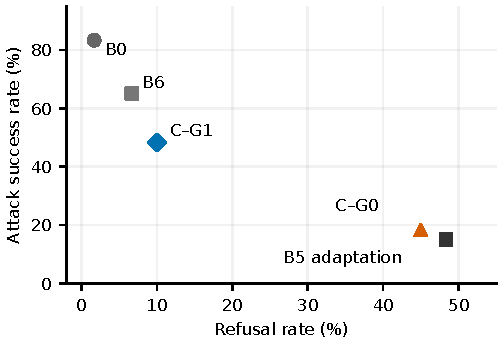
\includegraphics[width=\linewidth]{figures/tradeoff.pdf}
\caption{Measured operating points on the 60-query revised attacked evaluation. Lower values on both axes are preferable. Isolated points do not establish a calibrated frontier.}
\label{fig:tradeoff}
\Description{Scatter plot of attack success against refusal. B0 has high attack success and low refusal; C G1 is intermediate; C G0 and the B5 adaptation have lower attack success and higher refusal.}
\end{figure}

\subsection{Does Impact Contribute Beyond Other Features?}
\label{sec:ablation}
We distinguish feature removal from complete removal of Impact's eligibility dependency. C4 uses the four features and Equation~\ref{eq:gate}. C3-feature removes $I$ from the classifier but preserves that gate. C3-mechanism removes the classifier input and uses $g_h(C)=\mathbf{1}\{m\geq2,h(C)>0\}$. C4-$h$gate retains $I$ as an input but uses $g_h$. The latter isolates the gate change; it is not a size-only gate. Each classifier is retrained with the same seed set. Fixed-selector outcomes are summarized in Table~\ref{tab:ablation}.

\begin{table}[t]
\caption{Strict Impact ablation on 60 attacked validation queries. Fixed S2: $(\lambda,\tau)=(0.2,0.25)$; fixed S0: $\tau=0.5$. S0 columns give attack counts for the three training seeds.}
\label{tab:ablation}
\centering
\begin{tabular}{lcrrr}
\toprule
Variant & S2 ASR (\%) & \multicolumn{3}{c}{S0 attack count / 60}\\
 & All seeds & 20260825 & 42 & 7\\
\midrule
C4 & 66.7 & 14 & 14 & 14\\
C3-feature & 66.7 & 16 & 14 & 16\\
C3-mechanism & 66.7 & 15 & 16 & 13\\
C4-$h$gate & 66.7 & 15 & 15 & 14\\
\bottomrule
\end{tabular}
\end{table}

All twelve variant--seed combinations have S2 ASR 66.7\% and refusal 6.7\%. Thus the tested availability point shows no aggregate defensive gain from the Impact input or its eligibility dependency. Equal aggregate rates do not by themselves establish that all individual predictions are identical. At S0, C4 yields 14 attacks for each seed; the other variants yield 13--16. Their mean ASRs are 25.6\% for C3-feature and 24.4\% for both C3-mechanism and C4-$h$gate, compared with 23.3\% for C4. This small, seed-dependent separation is insufficient to support a stable mechanism claim. The seeds are repeated fits on the same queries, not three independent test samples.

These results are compatible with several explanations: the other structural features may already encode the relevant distinction, eligibility changes may rarely alter selections, or the retained-context policy may block additional deletions. The complete-coalition case described in Section~\ref{sec:method} establishes one such policy restriction, but the available aggregate ablation does not quantify its contribution to the observed equality. We retain Impact as an auxiliary engineering feature in the evaluated C4 configuration, not as an established source of improvement.

\subsection{Generation-Distribution Probes}
\label{sec:probe}
To compare graph support with generator behavior, we measure distributions with the full context and after coalition deletion. Let $y_{<t}$ be the same token prefix in both conditions, obtained from the full-context generation. For an available prefix length $T_q\leq H$, define
\begin{equation}
J_H(C)=\frac{1}{T_q}\sum_{t=1}^{T_q}\operatorname{JSD}\!\left(
P_\theta(\cdot\mid q,D,y_{<t}),
P_\theta(\cdot\mid q,D\setminus C,y_{<t})\right).
\label{eq:probe}
\end{equation}
The main maximum horizon is $H=16$, with $H=8$ and $32$ as sensitivity checks. Original token identities are retained for teacher forcing. The maximum horizon is not reached on every query: only 11 of the 63 coalition records have 16 available positions at $H=16$. For complete evidence removal, the second condition is a query-only generation probe, not the deployed selector's explicit refusal. Probing the distributions does not replace or modify the deployed refusal policy.

The completed summary contains 63 coalitions from 57 queries: 35 partial-evidence coalitions from 29 queries and 28 complete-evidence coalitions. For the 35 partial coalitions, the Pearson correlation of $I$ with $J_{16}$ is $0.2569$; Spearman correlation is $0.2835$. Table~\ref{tab:probe} gives the reported 95\% query-bootstrap interval, based on 1,000 resamples. The interval includes zero and spans both negative and moderately positive associations. This is insufficient validation of a reliable generation-effect proxy.

\begin{table}[t]
\caption{Impact--probe association by removal size at $H=16$. The 28 complete-evidence coalitions have constant Impact, so their within-group correlation is undefined. Intervals are reported query-bootstrap intervals.}
\label{tab:probe}
\centering
\begin{tabular}{lrrr}
\toprule
Removal group & Coalitions & Pearson $r$ & 95\% interval\\
\midrule
Partial, all sizes & 35 & 0.257 & $[-0.135,0.565]$\\
Size 2 & 16 & $-0.323$ & $[-0.691,0.299]$\\
Size 3 & 8 & 0.502 & $[0.050,0.962]$\\
Size 4 & 11 & $-0.330$ & $[-0.779,0.286]$\\
All evidence & 28 & Undefined & ---\\
\bottomrule
\end{tabular}
\end{table}

Stratification in Table~\ref{tab:probe} shows that the pooled positive association does not persist uniformly within deletion sizes. The positive size-three estimate is based on only eight coalitions; these exploratory subgroup intervals are not adjusted for multiple comparisons. Complete-evidence coalitions have mean probe divergence 0.4465, but all have $I=1$. Including their query-only probe values closes the measurement coverage gap; it cannot validate how Impact ranks effects within that group.

A disjoint same-size deletion control is available for 16 coalitions from 11 queries. Its mean divergence is 0.1208, compared with 0.1248 for coalition deletion. The paired difference is 0.0040, with reported query-bootstrap interval $[-0.0205,0.0373]$. This restricted comparison provides no clear evidence of excess influence beyond deletion size. It does not cover large coalitions for which the complement is too small to provide a disjoint control. Across all 63 coalitions, probe values at $H=8$ and $32$ correlate with $H=16$ at 0.9796 and 0.9897. That agreement concerns horizon sensitivity of the probe, not validity of Impact.

Finally, $J_H$ measures a distribution change along one fixed prefix. It is neither a comparison of two freely generated trajectories nor a directional measure of factual harm. Large divergence can result from removing useful evidence, and small divergence can coexist with an unchanged wrong answer. The probe and ablation together motivate treating Impact as graph-support sensitivity with an unvalidated relation to generation effects.

\subsection{Clean Availability and Answer Scores}
\begin{table}[t]
\caption{Clean evaluation: refusal counts out of 300 per dataset, and out of 900 overall. Gold answers are available for the HotpotQA evaluation subset only.}
\label{tab:clean}
\centering
\begin{tabular}{lrrr}
\toprule
Dataset & B0 & C--G1 & C--G0\\
\midrule
NQ & 37 & 38 & 38\\
HotpotQA & 200 & 200 & 200\\
MS MARCO & 20 & 27 & 36\\
Overall & 257 & 265 & 274\\
Overall refusal (\%) & 28.56 & 29.44 & 30.44\\
HotpotQA ESM (\%) & 11.33 & 11.33 & 11.33\\
HotpotQA token F1 & 0.1742 & 0.1742 & 0.1742\\
\bottomrule
\end{tabular}
\end{table}
Across the clean evaluation pool, G1 adds eight refusals and G0 adds seventeen (Table~\ref{tab:clean}). The increases are concentrated in MS MARCO. These aggregate increases should not be described as zero availability cost. Neither the misfilter budget nor the retention floor guarantees a fixed refusal rate.

On the 300 gold-available HotpotQA queries, all three methods have 34 exact-string matches and reported mean token F1 of 0.1742. Thus the available answer-quality measurement detects no degradation on this subset. It does not establish clean-answer preservation across all 900 queries. Moreover, the baseline itself refuses 200 of the 300 HotpotQA queries, and its low answer scores constrain the utility of an unchanged result. We do not infer practical adequacy or statistical equivalence from equality of these aggregate scores. The absent NQ and MS MARCO gold labels prevent answer-quality conclusions on those datasets.

\subsection{Transfer Across Generators}
\begin{table}[t]
\caption{Frozen C--G1 transfer on the 60-query attacked validation pool. Entries are percentages, shown as B0 $\rightarrow$ C--G1. No generator-specific retuning or independent transfer test is claimed.}
\label{tab:transfer}
\centering
\begin{tabular}{lrr}
\toprule
Generator & ASR (\%) & Refusal (\%)\\
\midrule
Qwen2.5-7B & $85.0\rightarrow66.7$ & $0.0\rightarrow6.7$\\
Llama-3.1-8B & $70.0\rightarrow56.7$ & $10.0\rightarrow13.3$\\
Mistral-7B-v0.3 & $88.3\rightarrow68.3$ & $0.0\rightarrow0.0$\\
\bottomrule
\end{tabular}
\end{table}
The ASR reduction has the same direction for all three generators (Table~\ref{tab:transfer}). However, Llama's refusal rate rises to 13.3\%, exceeding the 10\% budget used to select the Qwen operating point. The ASR reduction transfers in direction, but the availability constraint does not always transfer. The same small, development-used query pool and the similar generator scale limit broader conclusions.

\section{Discussion and Limitations}
The principal result is a trade-off between suppressing target answers and preserving availability. The availability point achieves a larger answer-match count than no filtering in the revised evaluation, while the protection point exchanges many potential answers for refusals. Neither operating point is an unconditional recommendation: deployment depends on how the application values wrong answers and unavailable answers. The current experiment does not estimate those application-specific costs.

Several limitations bound the claim. First, semantic grouping does not distinguish collusion from legitimate repetition or establish independent evidence. Leading-excerpt truncation and noisy NLI can miss contradictions or create spurious groups. Singletons are not scored, and S2 cannot remove an all-evidence coalition. Second, all attacked results use a five-passage retrieval setting and one targeted synthetic attack construction. The available family-level records do not establish separate, reproducible corpus snapshots, and the feedback-attack record is incomplete. We therefore make no validated family-generalization, adaptive-attack, or adversarial-training claim.

Third, the revised attacked pool was used during development, and the generator-transfer results reuse validation queries. There is no attacked independent confirmation reported here. Fourth, B5 is a project adaptation without a matched-refusal operating curve, and clean-answer labels cover only one dataset. Fifth, the newest ablation and probe findings are available as aggregate records; their per-query traces are absent from the accompanying archive. This limits independent checks of intervals and per-query transitions. Older traces from a different snapshot cannot fill that gap. Finally, timing summaries cover warm batches. End-to-end online latency was not measured.

For autonomous agents, the contribution concerns filtering external evidence before it is consumed. It does not demonstrate safer tool use or improved completion of agent tasks. A document coalition should not be read as a multiagent interaction merely because the filter is applicable upstream of an agent. These boundaries separate the implemented mechanism from applications that remain unevaluated.

\section{Conclusion}
We presented RAG-ConGuard, a coalition-level evidence filter with two explicit context-selection policies. In the examined targeted-poisoning setting, it reduces attack success relative to no filtering while exposing a substantial safety--availability trade-off. The available TrustRAG comparison does not establish superiority, and unchanged clean-answer scores are observed only on the labeled HotpotQA subset. The ablations and probes do not establish an Impact benefit at the availability point or validate it as a proxy for generation effects. Accordingly, the contribution is coalition-level evidence filtering and its measured operating trade-offs, with Impact retained as an auxiliary graph-support feature. The findings remain exploratory.

\paragraph{AI assistance.}
Use of ChatGPT, Codex, and Claude is disclosed in the supplement.

\clearpage
\balance
\bibliographystyle{ACM-Reference-Format}
\bibliography{references}
\end{document}
